% Desenvolvimento
O principal método de otimização desenvolvido a fim de solucionar os problemas de programação quadrática é o método de Newton que busca uma aproximação de segunda ordem da função objetivo por meio da série de Taylor. Este método, considerando funções perfeitamente quadrática, possui convergência rápida. Todavia, devido a necessidade de determinar a derivada de primeira e de segunda ordem da função objetivo, o seu esforço computacional pode ser elevado. Além disso, em muitos casos os problemas são considerados uma caixa preta, ou seja, a função objetivo não está disponível; e em outros casos, mesmo a função objetivo estando disponível, o cálculo de suas derivadas de primeira e de segunda ordem é uma operação extremamente complexa. Isso implica na utilização de métodos numéricos para a determinação das derivadas, acarretando em um custo computacional ainda mais elevado.
Todo esse cenário proporcionou o desenvolvimento de novos métodos de otimização, que buscam manter a qualidade de convergência do método de Newton e, simultaneamente, diminuir o custo computacional por meio de calcular as derivadas da função objetivo de forma aproximada. Como já abordado nesse trabalho, esses métodos são conhecidos como métodos Quase-Newton.
A fim de verificar e comparar o desempenho dos algoritmos da família de métodos Quase-Newton (o BFGS e o DFP nas suas formas tradicionais e com as adaptações de Huang e de Biggs) serão consideradas seis funções de teste, as quais são apresentadas nas próximas seções.

\subsection{Primeira Função de Teste}\label{sec:prifun}

A primeira função de teste se trata de uma função objetivo com variável de decisão e de dimensão dada por:

\begin{equation}\label{eq:prifuntst}
  f(x)= \frac{1}{2}*(x-c)^{T}*A*(x-c)
\end{equation}

Onde $c$ é um vetor unitário e $A$ é uma matriz diagonal. Ressalta-se que para os casos estudados é a matriz identidade. Esses parâmetros são apresentados abaixo:

\begin{equation*}
    X_{1xn} = \begin{bmatrix}
                    X_1 & X_2 & \ldots & X_n
                \end{bmatrix}    
\end{equation*}
\begin{equation*}
    C_{1xn} = \begin{bmatrix}
                    1 & 1 & \ldots & 1
                \end{bmatrix}    
\end{equation*}
\begin{equation*}
    A_{nxn} = \begin{bmatrix}
                    1 & 0 & \ldots & 0 & 0 \\
                    0 & 1 & \ldots & 0 & 0 \\
                    \vdots & \vdots & \ddots & \vdots & \vdots \\
                    0 & 0 & \ldots & 1 & 0 \\
                    0 & 0 & \ldots & 0 & 1 \\
                \end{bmatrix}    
\end{equation*}

O gradiente da função apresentada em \ref{eq:prifuntst} é dado por:

\begin{equation}\label{eq:gradprifuntst}
    \nabla f(x) = A*(x-c)
\end{equation}

Os gráficos dessa função, do gradiente e das curvas de nível considerando duas variáveis são ilustrados abaixo:

\begin{figure}[h!]
    \centering 
    \subfloat[][Função objetivo]{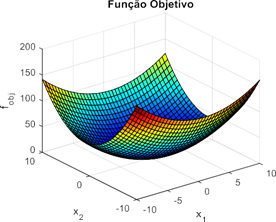
\includegraphics[scale=1]{img/section2/prifun.png}}    
    \qquad
    \subfloat[][Gradiente da função objetivo]{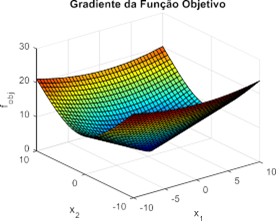
\includegraphics[scale=1]{img/section2/graprifun.png}} 
    \qquad
    \subfloat[][Curvas de nível]{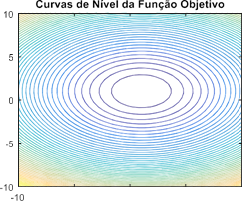
\includegraphics[scale=1]{img/section2/nivelprifun.png}} 
    \caption{Primeira função de teste}%
    \label{fig:prifun}%
\end{figure}
 \FloatBarrier
Ao observar os gráficos ilustrados nas figuras 1 e 2 é fácil notar que a função apresentada em \ref{eq:prifuntst} é uma função quadrática deslocada com o mínimo posicionado em $X_{1xn}=[\ 1 , 1 , \ldots , 1 ]\ $ (em duas dimensões um paraboloide).

\subsection{Segunda Função de Teste}\label{sec:secfun}

A segunda função de teste se trata de uma função objetivo com duas variáveis independentes com termos quadráticos e um cúbico, em que o termo cúbico deve apresentar menor influência no caso de se utilizar métodos Quase-Newton para determinar o mínimo da função. Essa função é definida como apresentado abaixo:

\begin{equation}\label{eq:secfuntst}
  f(x) = 12*x_1^2 - 4*x_2^2 - 12*x_1x_2 + 2*x_1 + a*(x_1^3+x_2^3)
\end{equation}

onde $a$ é um parâmetro que assume valores que ponderam a influência do termo cúbico na função. O gradiente da função apresentada em \ref{eq:secfuntst} pode ser escrito como se segue:

\begin{equation}\label{eq:gradsecfuntst}
    \nabla f(x) = \begin{cases}
        24*x_1-12*x_2+2+3*a*x_1^2\\
       8*x_2-12*x_1+3*a*x_2^2
    \end{cases}
\end{equation}

A solução ótima desse problema pode ser determinada ao considerar $\nabla f(x)=0$. Nesse caso, conforme pode ser observado pelo sistema de equações em \ref{eq:gradsecfuntst}, a solução ótima é dependente da escolha de $a$ , podendo ser obtida por meio da resolução desse sistema.
Os gráficos da função em \ref{eq:secfuntst}, do gradiente e das curvas de nível considerando valores do parâmetro $a$ igual a zero e igual a um são ilustrados abaixo:

\begin{figure}[h!]
    \centering 
    \subfloat[][Função objetivo]{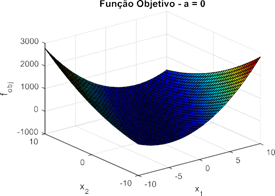
\includegraphics[scale=1]{img/section2/secfun0.png}}    
    \qquad
    \subfloat[][Gradiente da função objetivo]{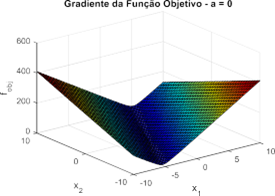
\includegraphics[scale=1]{img/section2/grasecfun0.png}}
    \qquad
    \subfloat[][Curvas de nível]{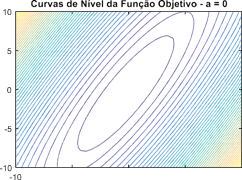
\includegraphics[scale=1]{img/section2/nivelsecfun0.png}}
    \caption{Segunda função de teste para $\alpha$=0}%
    \label{fig:secfun0}%
\end{figure}
\FloatBarrier

\begin{figure}[h!]
    \centering 
    \subfloat[][Função objetivo]{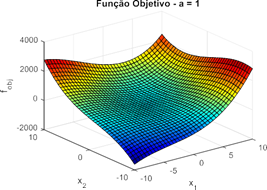
\includegraphics[scale=1]{img/section2/secfun1.png}}   
    \qquad
    \subfloat[][Gradiente da função objetivo]{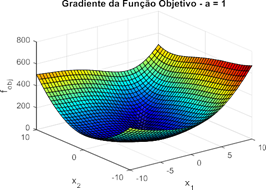
\includegraphics[scale=1]{img/section2/grasecfun1.png}}
    \qquad
    \subfloat[][Curvas de nível]{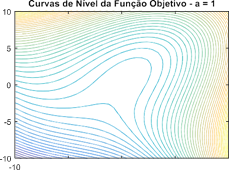
\includegraphics[scale=1]{img/section2/nivelsecfun1.png}}
    \caption{Segunda função de teste para $\alpha$=1}%
    \label{fig:secfun1}%
\end{figure}
\FloatBarrier

Ao observar os gráficos ilustrados nas figura \ref{fig:secfun0} nota-se que a função apresentada em \ref{eq:secfuntst} é uma função quadrática com o mínimo igual a $X =[\ -\frac{1}{3} , -\frac{1}{2} ]\ $. Já os gráficos ilustrados na figura \ref{fig:secfun1} mostram que esta mesma função é uma função não quadrática perfeita devido ao parâmetro não nulo (nesse caso,$a=1$). Além disso, o mínimo dessa função, como já mencionado, depende do parâmetro $a$.
Percebe-se que um importante aspecto relacionado à análise da função estudada é relativo ao intervalo de variação do parâmetro . Ressalta-se que somente para pequenos valores de $a$ ( faixa $-0.0263\leq a \leq 0.0263$ ) a Hessiana da função em \ref{eq:secfuntst} será semi-definida positiva, exceto no caso em que $a$ é nulo onde a Hessiana da função é definida positiva. Fora dessa faixa, ou seja, para valores de $a$ fora do intervalo, a função deixa de ser convexa. Nesse caso, o termo cúbico passa a ter maior influência e, consequentemente, no processo de busca de soluções pode ocorrer a convergência para bacias de atração indesejadas. Dessa forma, a faixa de variação do parâmetro $a$ deve ser dada de forma a respeitar a convexidade da função.
A matriz Hessiana da função estudada é apresentada pela equação abaixo:

\begin{equation}\label{eq:hessecfun}
    H = \begin{bmatrix}
                    24+6*a*x_1 & -12 \\
                    -12 & 8+6*a*x_2
                \end{bmatrix} \rightarrow det(H) = (24+6*a*x_1)*(8+6*a*x_2)-144   
\end{equation}

No caso em que a função em \ref{eq:secfuntst}  apresenta termos não quadráticos insignificativos, o determinante apresentado na equação \ref{eq:hessecfun} é diferente de zero. Já no caso contrário, o determinante se aproxima de zero, o que evidencia a singularidade da hessiana e a expressividade do termo não quadrático.

\subsection{Terceira Função de Teste}\label{sec:terfun}

A terceira função de teste se trata de uma função objetivo com duas variáveis de decisão como apresentado abaixo:

\begin{equation}\label{eq:terfuntst}
    f(x)=-8*x_1*x_2+\frac{4}{a^2}*x2*x2^3+\frac{4}{a^2}*x_1*x_2^3
\end{equation}

Ao observar a equação \ref{eq:terfuntst} percebe-se que a função objetivo $f(x)$ possui duas parcelas cúbicas. Todavia, ao considerar $a=\sqrt{2}$ e os intervalos para as variáveis de decisão igual a $[\ 0 , 3 ]\ $ tem-se  que a função $f(x)$ passa a se comportar como uma função quadrática. O gradiente da função apresentada em \ref{eq:terfuntst} pode ser escrito como segue:

\begin{equation}\label{eq:gradterfuntst}
    \nabla f(x) = \begin{cases}
         -8*x_2+\frac{12}{a^1}*x_2*x_1^2+\frac{4}{a^2}*x_2^3\\
         -8*x_1+\frac{12}{a^1}*x_1*x_2^2+\frac{4}{a^2}*x_1^3
    \end{cases}
\end{equation} 
   	   
Os gráficos dessa função, do gradiente e das curvas de nível considerando duas variáveis são ilustrados abaixo:

\begin{figure}[h!]
    \centering 
    \subfloat[][Função objetivo]{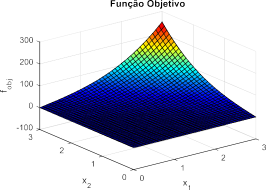
\includegraphics[scale=1]{img/section2/terfun.png}}   
    \qquad
    \subfloat[][Gradiente da função objetivo]{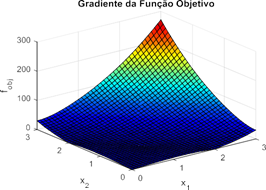
\includegraphics[scale=1]{img/section2/graterfun.png}}
    \qquad
    \subfloat[][Curvas de nível]{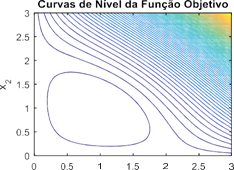
\includegraphics[scale=1]{img/section2/nivelterfun.png}}
    \caption{Terceira função de teste}%
    \label{fig:terfun}%
\end{figure}
\FloatBarrier

Ao observar os gráficos ilustrados na figura \ref{fig:terfun} observa-se que a função apresentada em (\ref{eq:terfuntst}), no intervalo definido para as variáveis de decisão, pode ser considerada uma função quadrática cujo o mínimo é dado pelo ponto $x=[\ 1 , 1 ]\ $.

\subsection{Quarta Função de Teste}\label{sec:quafun}

A quarta função de teste se trata de uma função objetivo com variável de decisão e de dimensão	dada por:

\begin{equation}\label{eq:quafuntst}
  f(x)= \frac{1}{2}*(x-c)^{T}*A*(x-c)+a*\sum_{k=1}^{n}{(x_k-1)^3}
\end{equation}


Onde $a$ é um parâmetro que pondera o termo cúbico,	$c$ é um vetor unitário e $A$ é uma matriz diagonal. Ressalta-se que para os casos estudados $A$ é a matriz identidade e $c$ é um vetor unitário como apresentado abaixo:

\begin{equation*}
    X_{1xn} = \begin{bmatrix}
                    X_1 & X_2 & \ldots & X_n
                \end{bmatrix}    
\end{equation*}
\begin{equation*}
    C_{1xn} = \begin{bmatrix}
                    1 & 1 & \ldots & 1
                \end{bmatrix}    
\end{equation*}
\begin{equation*}
    A_{nxn} = \begin{bmatrix}
                    1 & 0 & \ldots & 0 & 0 \\
                    0 & 1 & \ldots & 0 & 0 \\
                    \vdots & \vdots & \ddots & \vdots & \vdots \\
                    0 & 0 & \ldots & 1 & 0 \\
                    0 & 0 & \ldots & 0 & 1 \\
                \end{bmatrix}    
\end{equation*}

No caso em que o parâmetro $a$ é igual a zero, a função $f(x)$ se torna idêntica a primeira função de teste apresentada na seção \ref{sec:prifun}. Dessa forma, para o termo cúbico ser considerado, o valor de $a$ deve ser diferente de zero.
O gradiente da função apresentada em (\ref{eq:quafuntst}) é dado por:

\begin{equation}\label{eq:gradquafuntst}
    \nabla f(x) = A*(x-c)+3*a*\sum_{k=1}^{n}{(x_k-1)^2}
\end{equation}

A Hessiana dessa função é descrita como:

\begin{equation}\label{eq:hesquafuntst}
    H_{nxn} = \begin{bmatrix}
                    1+6*a(x_1-1) & 0            & \ldots & 0                & 0 \\
                    0            & 1+6*a(x_2-1) & \ldots & 0                & 0 \\
                    \vdots       & \vdots       & \ddots & \vdots           & \vdots \\
                    0            & 0            & \ldots & 1+6*a(x_{n-1}-1) & 0 \\
                    0            & 0            & \ldots & 0                & 1+6*a(x_{n}-1) \\
                \end{bmatrix}    
\end{equation}    
{\centering \\ $\downarrow$\\}
\begin{equation*}
det(H)=(1+6*a(x_1-1))*( 1+6*a(x_2-1))*\ldots*(1+6*a(x_{n-1}-1))*(1+6*a(x_{n}-1))
\end{equation*}

No intuito de obter uma Hessiana semi-definida positiva, ou seja, no caso onde não há singularidade, deve-se obter valores de que respeitem a seguinte condição: $det(H)\geq 0$.
O valor do parâmetro para função \ref{eq:gradquafuntst} foi $a = 0.0263$. 

Os gráficos dessa função, do gradiente e das curvas de nível considerando duas variáveis são ilustrados abaixo:

\begin{figure}[h!]
    \centering 
    \subfloat[][Função objetivo]{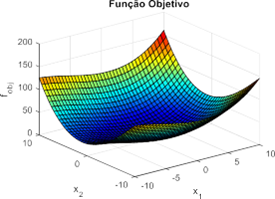
\includegraphics[scale=1]{img/section2/quafun.png}}
    \qquad
    \subfloat[][Gradiente da função objetivo]{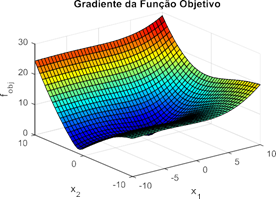
\includegraphics[scale=1]{img/section2/graquafun.png}}
    \qquad
    \subfloat[][Curvas de nível]{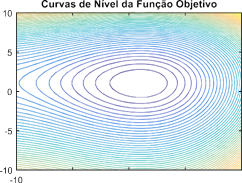
\includegraphics[scale=1]{img/section2/nivelquafun.png}}
    \caption{Quarta função de teste}%
    \label{fig:quafun}%
\end{figure}
\FloatBarrier

Ao observar os gráficos ilustrados nas figuras 9 e 10 é fácil notar que a função apresentada em (\ref{eq:quafuntst}) é uma função não quadrática perfeita devido ao parâmetro $a = 0.0263$, não nulo (nesse caso). Além disso, o mínimo dessa função depende do valor do parâmetro $a$.

\subsection{Quinta Função de Teste}\label{sec:quifun}

A quinta função de teste é uma função com duas variáveis proveniente do problema de Rosen-Suzuki. Esse problema é considerado um problema de otimização restrito cuja função pseudo-objetivo pode ser considerada uma função quadrática. Vale ressaltar que a função pseudo-objetivo é dada pela soma da função objetivo com a função de penalidade que traduz as restrições não lineares, fazendo com que as soluções fornecidas por algum processo de otimização sejam factíveis.\par
Os gráficos dessa função, do gradiente e das curvas de nível considerando duas variáveis são ilustrados abaixo:

\begin{figure}[h!]
    \centering 
    \subfloat[][Função objetivo]{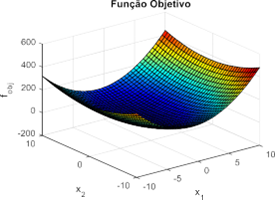
\includegraphics[scale=1]{img/section2/quifun.png}}   
    \qquad
    \subfloat[][Gradiente da função objetivo]{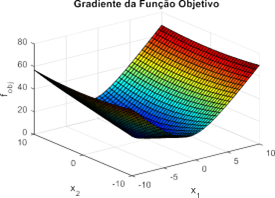
\includegraphics[scale=1]{img/section2/graquifun.png}}
    \qquad
    \subfloat[][Curvas de nível]{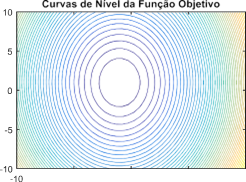
\includegraphics[scale=1]{img/section2/nivelquifun.png}}
    \caption{Quinta função de teste}%
    \label{fig:quifun}%
\end{figure}
\FloatBarrier

Ao observar os gráficos ilustrados nas figuras 11 e 12 nota-se que a função pseudo-objetivo do problema Rosen-Suzuki é uma função quadrática com o mínimo posicionado em $x=[\ -1 , 1 ]\ $.

\subsection{Sexta Função de Teste}\label{sec:sexfun}

A sexta e última função de teste a ser estudada nesse trabalho se trata de uma função objetivo com n variáveis de decisão conhecida como função de  norma condicionada e inclinada \textit{(tilted and conditioned norm)}. Essa função na sua forma geral é apresentada abaixo:

\begin{equation}\label{eq:sexfuntst}
  f(x)= w*\lVert A*x \rVert_p+(w-1)*(A*x)_1
\end{equation}

Sendo $w$ e $p$ parâmetros da função $f(x)$ e o índice 1 do termo $(A*x)$ indica que apenas o primeiro elemento desse produto escalar é considerado. Além disso, a matriz $A$ é uma matriz quadrada conhecida como matriz de Hilbert em que os seus elementos são calculados de acordo com a equação abaixo:

\begin{equation}\label{eq:auxsexfuntst}
  A(i,j)= \frac{1}{1+i-j} \begin{cases}
        i \rightarrow N\degree linha\\
        j \rightarrow N\degree Coluna
    \end{cases}
\end{equation}

Considerando $p=2$, $w=8$ e $x=[\ x_1 , x_2 ]\ $ (problema com duas dimensões), a equação (\ref{eq:sexfuntst}) pode ser escrita conforme apresentado abaixo:

\newcommand\norm[1]{\left\lVert#1\right\rVert}

\begin{equation}\label{eq:sexfuntst}
  f(x)= 8*\norm{ x_1 + \frac{x_2}{2},\frac{x_1}{2}+\frac{x_2}{3} }_2+7*(x_1+\frac{x_2}{2}) 
\end{equation}

No caso da equação apresentada em (\ref{eq:sexfuntst}), o operador $\norm{,}_2$  equivale à norma Euclidiana ($\mathbb{L}_2$). \par
O gradiente da função $f(x)$ na sua forma geral é dado por:

\begin{equation}\label{eq:gradsexfuntst}
    \nabla f(x) = \left(\frac{w*x^T*A^T*A}{\norm{A*x}_p}+(w-1)*(A*x)\right)^T
\end{equation}

Novamente, considerando $p=2$, $w=8$ e $x=[\ x_1 , x_2 ]\ $ (problema com duas dimensões), a equação (\ref{eq:gradsexfuntst}) pode ser escrita conforme apresentado abaixo:

\begin{equation}\label{eq:gradsexfuntst}
    \nabla f(x) = \left(\frac{8*x^T*A^T*A}{\norm{ x_1 + \frac{x_2}{2},\frac{x_1}{2}+\frac{x_2}{3} }_2}+7*(A*x)\right)^T
\end{equation}

Sendo:

\begin{equation*}
    A = \begin{bmatrix}
        1 & \frac{1}{2} \\
        \frac{1}{2} & \frac{1}{3} \\
    \end{bmatrix}
\end{equation*}

\begin{equation*}
    x = \begin{bmatrix}
        x_1 & x_2
    \end{bmatrix}
\end{equation*}

Essa função, além de não ser uma função quadrática, apresenta um comportamento cujo valor do determinante da Hessiana é muito próximo de zero. Dessa forma, é constatado um problema de otimização com singularidade, o qual os métodos Quase-Newton possuem dificuldades de resolver, tornando relevante o estudo de como esses métodos conseguem contornar esse problema. Vale ressaltar que a solução ótima, no caso da função objetivo escrita em (\ref{eq:sexfuntst}) é igual a $x=[\ 0 , 0 ]\ $. \par

Os gráficos da função apresentada nessa seção, do gradiente e das curvas de nível considerando duas variáveis são ilustrados abaixo:

\subsection{Considerações dos Experimentos}
  A Tabela \ref{tab:tab_doe} apresenta de forma sumarizada como os experimentos devem ser realizados e analisados.
  % Please add the following required packages to your document preamble:
% \usepackage{multirow}
% \usepackage{graphicx}
% \usepackage[table,xcdraw]{xcolor}
% If you use beamer only pass "xcolor=table" option, i.e. \documentclass[xcolor=table]{beamer}
\begin{table}[h!]
\resizebox{\textwidth}{!}{%
\begin{tabular}{c|cccccc|}
\cline{2-7}
 &
 \multicolumn{6}{c|}{\cellcolor[HTML]{EFEFEF}Experimentos} \\ \cline{2-7} 
\multirow{-2}{*}{} &
 \multicolumn{1}{c|}{\cellcolor[HTML]{EFEFEF}1º} &
 \multicolumn{1}{c|}{\cellcolor[HTML]{EFEFEF}2º} &
 \multicolumn{1}{c|}{\cellcolor[HTML]{EFEFEF}3º} &
 \multicolumn{1}{c|}{\cellcolor[HTML]{EFEFEF}4º} &
 \multicolumn{1}{c|}{\cellcolor[HTML]{EFEFEF}5º} &
 \cellcolor[HTML]{EFEFEF}6º \\ \hline
\multicolumn{1}{|c|}{\cellcolor[HTML]{EFEFEF}Descrissão} &
 \multicolumn{1}{c|}{\begin{tabular}[c]{@{}c@{}}Avaliação das \\ Funções \\ quadráticas\end{tabular}} &
 \multicolumn{1}{c|}{\begin{tabular}[c]{@{}c@{}}Avaliação das \\ funções não \\ quadráticas\end{tabular}} &
 \multicolumn{1}{c|}{\begin{tabular}[c]{@{}c@{}}Avaliação do \\ custo \\ computacional \\ em função da \\ variação da \\ dimensão\end{tabular}} &
 \multicolumn{1}{c|}{\begin{tabular}[c]{@{}c@{}}Técnica da Seção \\ Áurea Avaliação \\ direta da função e \\ aproximações \\ quadráticas da \\ função a cada \\ iteração\end{tabular}} &
 \multicolumn{1}{c|}{\begin{tabular}[c]{@{}c@{}}Avaliação dos \\ métodos Quase- \\ Newton em \\ problemas com \\ Hessiana singular\end{tabular}} &
 \begin{tabular}[c]{@{}c@{}}Avaliação \\ estatística \\ dos métodos \\ Quase \\ Newton com \\ a variação do \\ \textbf{Parâmetro} $\alpha$\end{tabular} \\ \hline
\multicolumn{1}{|c|}{\cellcolor[HTML]{EFEFEF}} &
 \multicolumn{1}{c|}{1ª Função de Teste} &
 \multicolumn{1}{c|}{} &
 \multicolumn{1}{c|}{} &
 \multicolumn{1}{c|}{4ª Função de Teste} &
 \multicolumn{1}{c|}{} &
  \\
\multicolumn{1}{|c|}{\cellcolor[HTML]{EFEFEF}} &
 \multicolumn{1}{c|}{2ª Função de Teste} &
 \multicolumn{1}{c|}{} &
 \multicolumn{1}{c|}{} &
 \multicolumn{1}{c|}{5º Função de Teste} &
 \multicolumn{1}{c|}{} &
  \\
\multicolumn{1}{|c|}{\multirow{-3}{*}{\cellcolor[HTML]{EFEFEF}\begin{tabular}[c]{@{}c@{}}Funções \\ Avaliadas\end{tabular}}} &
 \multicolumn{1}{c|}{3ª Função de Teste} &
 \multicolumn{1}{c|}{\multirow{-3}{*}{2ª Função de Teste}} &
 \multicolumn{1}{c|}{\multirow{-3}{*}{4ª Função de Teste}} &
 \multicolumn{1}{c|}{} &
 \multicolumn{1}{c|}{\multirow{-3}{*}{6º Função de Teste}} &
 \multirow{-3}{*}{2ª Função de Teste} \\ \hline
\multicolumn{1}{|c|}{\cellcolor[HTML]{EFEFEF}} &
 \multicolumn{1}{c|}{fex1} &
 \multicolumn{1}{c|}{} &
 \multicolumn{1}{c|}{} &
 \multicolumn{1}{c|}{fexLivro} &
 \multicolumn{1}{c|}{} &
  \\
\multicolumn{1}{|c|}{\cellcolor[HTML]{EFEFEF}} &
 \multicolumn{1}{c|}{fexLivro} &
 \multicolumn{1}{c|}{} &
 \multicolumn{1}{c|}{} &
 \multicolumn{1}{c|}{fex1} &
 \multicolumn{1}{c|}{} &
  \\
\multicolumn{1}{|c|}{\multirow{-3}{*}{\cellcolor[HTML]{EFEFEF}\begin{tabular}[c]{@{}c@{}}Código das \\ Funções Avaliadas \\ no Matlab\end{tabular}}} &
 \multicolumn{1}{c|}{fex3} &
 \multicolumn{1}{c|}{\multirow{-3}{*}{fexLivro}} &
 \multicolumn{1}{c|}{\multirow{-3}{*}{fex1}} &
 \multicolumn{1}{c|}{fun\_rosensuzuki\_irr} &
 \multicolumn{1}{c|}{\multirow{-3}{*}{f\_tiltednormcond}} &
 \multirow{-3}{*}{fexLivro} \\ \hline
\end{tabular}%
}
\caption{Detalhamento dos experimentos realizados para as análises dos Métodos Quase-Newton.}
\label{tab:tab_doe}
\end{table}

Nos experimentos realizados nesse trabalho alguns Parâmetros devem ser fixados a fim executar os algoritmos desenvolvidos em ambiente Matlab e possibilitar uma análise adequada. A descrição de tais Parâmetros de uma forma geral e mais especifica, considerando os experimentos, é apresentada abaixo:
\begin{itemize}
  \item \textbf{Parâmetro}: $Imetqn\rightarrow$ Chaveia o algoritmo Quase-Newton a ser executado
  \item \textbf{Parâmetro}: $icaso\rightarrow$ Chaveia a função objetivo a ser estudada
  \item \textbf{Parâmetro}: $a\rightarrow$ Pondera os termos não quadráticos
  \item \textbf{Parâmetro}: $dim\rightarrow$ Determina a dimensão do problema a ser resolvido
  \item \textbf{Parâmetro}: $xstar\rightarrow$ Estabelece a solução ótima do problema
  \item \textbf{Parâmetro}: $x0\rightarrow$ Estabelece o ponto inicial
  \item \textbf{Parâmetro}: $isa\_FV\rightarrow$ Chaveia a técnica da Seção Áurea
\end{itemize}

A função desenvolvida no Matlab que soluciona os problemas propostos nesse trabalho é codificada como \textbf{otqnmat\_a77}. Os parâmetros dessa função são pontuados a seguir:

\begin{itemize}
  \item \textbf{Parâmetro de entrada}: $funcao\rightarrow$ Função a ser aproximada
  \item \textbf{Parâmetro de entrada}: $isa\_FV\rightarrow$ Seção Áurea
  \item \textbf{Parâmetro de entrada}: $Imetqn\rightarrow$ Método Quase-Newton escolhido 
  \item \textbf{Parâmetro de entrada}: $MAXITER\rightarrow$ Número máximo de iterações 
  \item \textbf{Parâmetro de entrada}: $x0\rightarrow$ Ponto inicial
  \item \textbf{Parâmetro de entrada}: $xMin\rightarrow$ Limite inferior 
  \item \textbf{Parâmetro de entrada}: $xMAx\rightarrow$ Limite superior 
  \item \textbf{Parâmetro de entrada}: $epslon\rightarrow$ Precisão
  \item \textbf{Parâmetro de saída}: $XK1\rightarrow$ Armazena a solução das variáveis de decisão 
  \item \textbf{Parâmetro de saída}: $Hfobjrightarrow$ Armazena os valores da função objetivo 
  \item \textbf{Parâmetro de saída}: $icfunc\rightarrow$ Número de avaliações da função objetivo
\end{itemize}

Finalmente, a precisão que define um dos critérios de parada dos algoritmos Quase-Newton executados nesse trabalho será $10^{-6}$ . Sendo \textbf{dim} a dimensão do problema de otimização a ser resolvido. O número máximo de iterações define um segundo critério de parada e será:

\begin{equation}\label{eq:maxevals}
    \textrm{N\degree Máximo de Iteração} = 2 * dim * 100    
\end{equation}

\newpage